\documentclass[12pt]{article}
\usepackage[margin=1in]{geometry}
\geometry{letterpaper}                  
\usepackage{graphicx}
\usepackage[hyphens]{url}
\usepackage{fancyhdr}
\pagestyle{fancy}
\usepackage{fixltx2e}
\usepackage{amsmath,amsfonts,amsthm,amssymb}
\usepackage{graphicx}
\usepackage{algorithm}
\usepackage{algorithmic}
\usepackage{url}
\usepackage[normalem]{ulem}
\usepackage[pdftex]{color}
\usepackage{varioref}
\usepackage{mathrsfs}
\usepackage{amsmath}
\labelformat{equation}{\textup{(#1)}}
\usepackage[sort&compress,colon,square,numbers]{natbib}


\usepackage{color}
\newcommand{\todo}[1]{{\color{red}{\it TODO: #1}}}
\newcommand{\jovo}[1]{{\color{green}{\it jovo: #1}}}
\newcommand{\will}[1]{{\color{blue}{\it will: #1}}}
\newcommand{\greg}[1]{{\color{cyan}{\it greg: #1}}}


\begin{document}

\begin{center}\Large \bf EN.580.694: Statistical Connectomics \\ Final Project: Redefining Bock \end{center}
\begin{center} Erika Dunn-Weiss $\cdot$  \today \end{center}
\bigskip


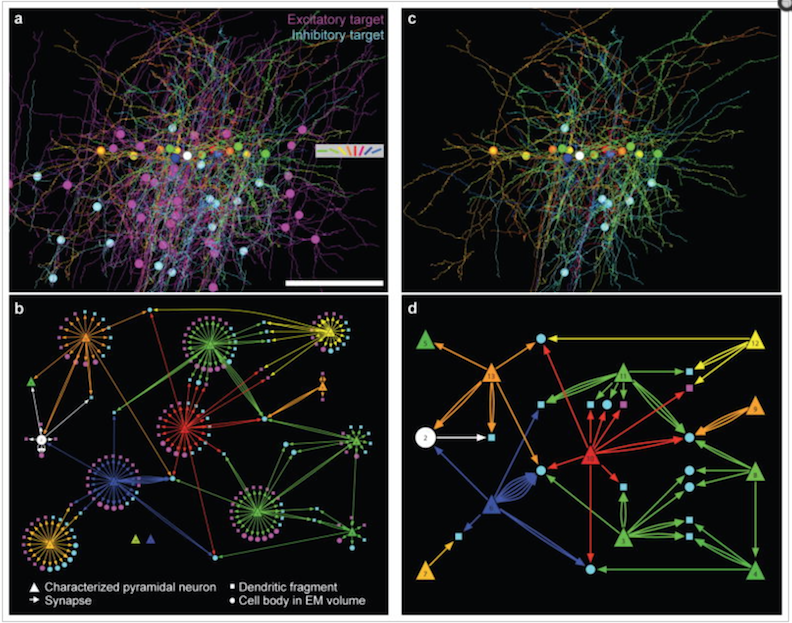
\includegraphics{OriginalBockGraphs.png}
\bigskip

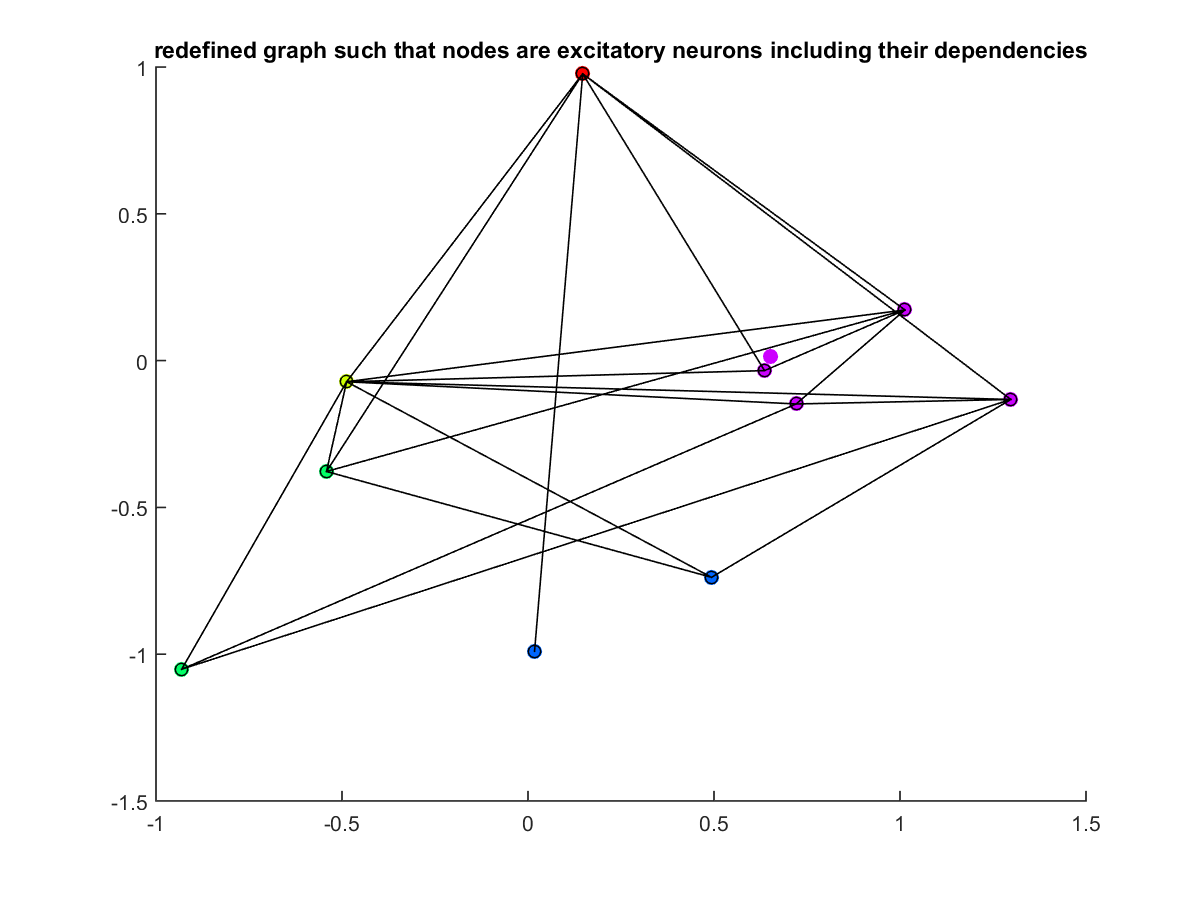
\includegraphics{redefinedGraph.png}

\section*{Opportunity}  In the Bock paper, Bock et al. attempted to answer the question: do inhibitory interneurons in the mouse primary visual cortex receive convergent input from excitatory pyramidal neurons with similar or varying preferred stimulus orientation? However, in defining the graph where nodes are neurons and edges are synapses between those neurons, they could not use a Stochastic Block Model (SBM) to answer their question: a SBM cannot help answer questions pertaining to relationships between three nodes. 

\section*{Challenge} The challenge was to redefine the graph so that the question above could be answered using a SBM.

\section*{Action} The idea was to redefine the graph so that the nodes now contain information about their dependencies, i.e. their Markov blanket. Consider the simple case of two excitatory neurons synapsing onto an inhibitory neuron. Previously, the attributes of the excitatory neurons as nodes were simply that they were excitatory and their preferred orientation. Now, we again set nodes to be neurons but this time we only consider excitatory neurons as nodes, and we include as a node attribute the inhibitory neuron that the excitatory neuron synapsed onto, this being part of its Markov blanket. Now that nodes contain this dependency, we can define an edge between two nodes when the nodes contain the same inhibitory neuron attribute: i.e. that they synapse onto the same inhibitory neuron. 

Once we have redefined the graph this way, we use a SBM with known clusters, where the clusters are the orientation preferences of the excitatory neurons. The test statistic is that the probability of an edge within clusters, $p$ minus the probability of an edge between clusters $q$. This is a special class of SBM called an affinity model. The null hypothesis is that $p-q$ $\textgreater$ 0, which we wish to reject in favor of $p-q$ $\leq$ 0, i.e., that inhibitory neurons do intact get convergent input from pyramidal neurons with widely varying preferred stimulus orientations. 

\section*{Resolution} 

In fact, we do observe $H_a$ in that $p-q$ = -0.7143. To test the significance of this, we do a permutation test with 10,000 permutations. Unfortunately, the result is not significant, $p$ $\textgreater$ 0.5. 

\section*{Future} 
Limitations of this are that the graph is quite small, especially once redefined: it only consists of 11 nodes and 42 edges. Furthermore, the affinity block model raises the issue that the variance of $q$ is much smaller than the variance of $p$. There may be a better method with higher power to evaluate this test statistic that takes into account the difference in variances. It would also be useful in general to follow up with a power analysis as a function of the test statistic $p-q$ and the sample size $n$ to get a sense of both of these limitations. 

\section*{Additional notes}
The graph in .m form was provided with assistance from Greg Kiar's code to convert graphML to mat files. The graph attributes, i.e. orientation preferences of the neurons and whether or not they were inhibitory or excitatory etc. were hand characterized using the attributes from the graph ML file and heavily relying on the graphs depicted in the Bock 2011 paper where there is a color scale for orientation tuning and neurons are color coded accordingly. 

\newpage

Thank you for a great class! Please let me know if there's an opportunity to do more with this!
\section*{References}
\bibliography{Bock}
Bock DD, Lee WC, Kerlin AM, Andermann ML, Hood G, Wetzel AW, Yurgenson S, Soucy ER, Kim HS, Reid RC.
Nature. 2011 Mar 10;471(7337):177-82. doi: 10.1038/nature09802.
PMID: 21390124
\end{document}  